\begin{figure}[H]
\begin{center}
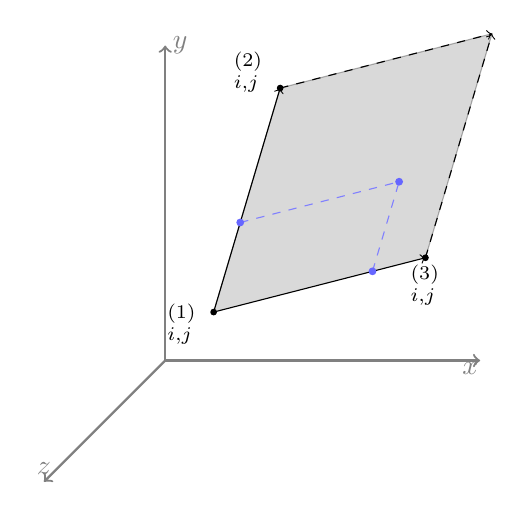
\begin{tikzpicture}

%   \draw[fill=gray!20, opacity=0.6] (3,3,3) -- (2,3,3) -- (2,2,3) -- (3,2,3); % przod 
%   \draw[fill=gray!45, opacity=0.6] (3,3,3) -- (2,3,3) -- (2,3,2) -- (3,3,2); % gora 
%   \draw[fill=gray!60, opacity=0.9] (3,3,3) -- (3,3,2) -- (3,2,2) -- (3,2,3); % prawy bok 
%   \draw[fill=gray!30, opacity=0.6] (3,2,3) -- (2,2,3) -- (2,2,2) -- (3,2,2); % dol
%   \draw[fill=gray!10, opacity=0.5] (2,3,3) -- (2,3,2) -- (2,2,2) -- (2,2,3); % lewy  bok 
%   \draw[fill=gray!15, opacity=0.8] (3,3,2) -- (2,3,2) -- (2,2,2) -- (3,2,2); % przod
  
  
%   
  \draw[thick,->, color=gray] (0,0,0) -- (4,0,0) node[below left=-3]{$x$};
  \draw[thick,->, color=gray] (0,0,0) -- (0,4,0) node[right=-1]{$y$};
  \draw[thick,->, color=gray] (0,0,0) -- (0,0,4) node[above=-1]{$z$};
  
%   

%    \draw (3,0,0) coordinate (x) |- (0,3,0) coordinate [midway] (h) coordinate (y) -- (0,3,3) coordinate (a) -- (0,0,3) coordinate (z) -- (3,0,3) edge (x) -- (3,3,3) coordinate (v) edge (h)
%    -- (a)  ;
% %   
%    \draw [dashed, color=gray] (0,0,0) coordinate (o) edge (x) edge (y) -- (z);
  
  %\draw[->,color=red] (x) -- (o);
 
  \coordinate  (q1) at (1,1,1) ;
   \coordinate  (q2) at (3,5,4);
    \coordinate  (q3) at (6,4,7);
    \coordinate  (q4) at (8,8,10);
    
    
 
  \draw[fill=gray,opacity=0.3] (q1)--(q2)--(q4) --(q3);
  
  
    \draw[->] (q1) -- (q2);
    
    \draw[->] (q1) -- (q3);
  
  \draw[->,dashed] (q2) -- (q4);
  \draw[->,dashed] (q3) -- (q4);
  
  \draw plot [mark=*, mark size=1] coordinates{(q1)}; 
  \draw plot [mark=*, mark size=1] coordinates{(q2)}; 
  \draw plot [mark=*, mark size=1] coordinates{(q3)}; 
  
   \node  at (0.6,0.85, 1) {$\bfq_{i,j}^{(1)}$};
   
     \node  at (2.6,5.2, 4) {$\bfq_{i,j}^{(2)}$};
     
       \node  at (6,3.65, 7) {$\bfq_{i,j}^{(3)}$};

   \coordinate  (R1) at (1.8,2.6,2.2);
   \coordinate   (R2) at (4.75,3.25, 5.5);
   \coordinate  (R3) at (5.55,4.85, 6.7);
   
%   \draw plot [mark=*, mark size=1,fill=red] coordinates{(R1)}; 
%   \draw plot [mark=*, mark size=1] coordinates{(R2)}; 
%   \draw plot [mark=*, mark size=1] coordinates{(R3)}; 
  
  \draw[dashed, color=gray!75,color=blue!50] (R1) -- (R3);
  \draw[dashed, color=gray!75,color=blue!50] (R2) -- (R3);
  
   
     \node[color=blue!75]  at (5.5,5.11, 6.9) {$\bfp$};
     
  \node at (R1) [circle,fill=blue!60,inner sep=1pt]{};
  \node at (R2) [circle,fill=blue!60,inner sep=1pt]{};
  \node at (R3) [circle,fill=blue!60,inner sep=1pt]{};
  
  
  
  
% 
%   \draw (1,0,3) -- (1,3,3) -- (1,3,0);
%   \draw (2,0,3) -- (2,3,3) -- (2,3,0);
%   
%   \draw (0,3,1) -- (3,3,1) -- (3,0,1);
%   \draw (0,3,2) -- (3,3,2) -- (3,0,2);
%   
%   
%   \draw (0,1,3) -- (3,1,3) -- (3,1,0);
%   \draw (0,2,3) -- (3,2,3) -- (3,2,0);
%   
%   
%   \draw [dashed, color=gray] (1,0,1) -- (1,3,1) ;
%   \draw [dashed, color=gray] (1,0,2) -- (1,3,2) ;
%   
%   \draw [dashed, color=gray] (2,0,1) -- (2,3,1);  
%   \draw [dashed, color=gray] (2,0,2) -- (2,3,2) ; 
%   
%   \draw [dashed, color=gray] (0,3,1) -- (0,0,1) -- (3,0,1);  
%   \draw [dashed, color=gray] (0,3,2) -- (0,0,2) -- (3,0,2);  
%   
%   \draw [dashed, color=gray] (1,0,3) -- (1,0,0) -- (1,3,0);  
%   \draw [dashed, color=gray] (2,0,3) -- (2,0,0) -- (2,3,0);  
%   
%   \draw [dashed, color=gray] (0,1,0) -- (3,1,0);
%   \draw [dashed, color=gray] (0,1,1) -- (3,1,1);
%   \draw [dashed, color=gray] (0,1,2) -- (3,1,2);
%   
%   \draw [dashed, color=gray] (0,2,0) -- (3,2,0);
%   \draw [dashed, color=gray] (0,2,1) -- (3,2,1);
%   \draw [dashed, color=gray] (0,2,2) -- (3,2,2);
%   
%   \draw [dashed, color=gray] (1,1,3) -- (1,1,0);
%   \draw [dashed, color=gray] (2,1,3) -- (2,1,0);
%   
%   \draw [dashed, color=gray] (1,2,3) -- (1,2,0);
%   \draw [dashed, color=gray] (2,2,3) -- (2,2,0);
%   
%   \draw [dashed, color=gray] (0,1,3) -- (0,1,0) ;
%   \draw [dashed, color=gray] (0,2,3) -- (0,2,0) ;
%   
%   \node [circle, minimum size=4pt, inner sep=0pt, fill, label=0:$\bfu_3$] at (2.4, 2.19, 2.1) {};
%   \node [circle, minimum size=4pt, inner sep=0pt, fill, label=0:$\bfu_7$] at (2.1, 2.6, 2.35) {};
%   \draw [->] (x) -- +(1pt,0,0) node [midway,above] {$x$};
%   \draw [->] (y) -- +(0,1pt,0) node [midway,right] {$y$};
%   \draw [->] (z) -- +(0,0,1pt) node [midway,above] {$z$};
 
 \end{tikzpicture}
\caption{A parallelogram span over $\bfq_{i,j}^{(1)}=(1,1,1), \bfq_{i,j}^{(2)}=(3,5,4), 
\bfq_{i,j}^{(3)}=(6,4,7).$ Points chosen uniformly on $(\bfq_{i,j}^{(1)},\bfq_{i,j}^{(2)})$ and 
on $(\bfq_{i,j}^{(1)},\bfq_{i,j}^{(3)})$ and resulting random point in a 
parallelogram depicted.}
\label{fig:parallelogram}
\end{center}
\end{figure}
